\documentclass[12pt,letterpaper]{article}

% ── Packages ──────────────────────────────────────────────────────────────────
\usepackage[margin=1in]{geometry}
\usepackage{amsmath,amssymb}
\usepackage{natbib}
\usepackage{graphicx}
\usepackage{booktabs}
\usepackage{tabularx}
\usepackage{float}
\usepackage{hyperref}
\usepackage{setspace}
\usepackage[labelfont=bf]{caption}
\usepackage{subcaption}
\usepackage{enumitem}

\doublespacing
\hypersetup{colorlinks=true, linkcolor=blue, citecolor=blue, urlcolor=blue}

% ── Title ─────────────────────────────────────────────────────────────────────
\title{%
  Climate, Crops, and the Malthusian Trap:\\
  Agricultural Transition Pathways and Population Dynamics\\
  from Antiquity to the Early Modern Period%
}
\author{
  [Author Name]\\
  \textit{[Affiliation]}\\
  \texttt{[email]}
}
\date{Draft: April 2026}

\begin{document}
\maketitle

\begin{abstract}
\noindent
We use HYDE~3.5 historical land-use and population data (10,000~BCE--2025~CE) combined with ERA5 reanalysis climate data to investigate the mechanisms of Malthusian population dynamics across 197 countries. We document three sets of findings. First, we identify five distinct agricultural transition pathways---high-density intensive, early extensifiers, crop-dominant late developers, pastoral/mixed late developers, and irrigation pioneers---that exhibit fundamentally different Malthusian dynamics. Second, using climate-determined crop composition as instruments for agricultural productivity, we show that OLS estimates of the agricultural productivity--population growth relationship are biased downward by reverse causality; the IV estimate reveals a positive causal effect of exogenous productivity gains on population growth, consistent with the core Malthusian mechanism. Third, we establish ``iron laws'' of climate--agriculture linkages: temperature shocks reduce agricultural land growth ($\beta = -0.012$, $p = 0.01$), crop-dominant economies are significantly more climate-resilient than pastoral ones (7.7$\times$ less sensitive), and warming paradoxically increases population growth despite reducing agricultural output. The Manski bounds on the Malthusian coefficient are entirely negative across all HYDE uncertainty scenarios, confirming robustness to measurement error in historical data.

\vspace{0.5em}
\noindent\textbf{JEL Codes:} N50, O13, O44, Q54, J11\\
\textbf{Keywords:} Malthusian trap, unified growth theory, agricultural transition, climate shocks, instrumental variables, HYDE~3.5
\end{abstract}

\newpage
\tableofcontents
\newpage

% ══════════════════════════════════════════════════════════════════════════════
\section{Introduction}
% ══════════════════════════════════════════════════════════════════════════════

The Malthusian model---in which population growth absorbs productivity gains, preventing sustained increases in living standards---remains the dominant framework for understanding pre-industrial economic dynamics \citep{galor2011unified, ashraf2011dynamics}. Yet the empirical evidence for Malthusian mechanics has relied on either highly aggregated cross-country comparisons or detailed case studies of individual societies. The mechanisms by which different agricultural systems mediated the relationship between climate, productivity, and population remain poorly understood.

This paper exploits the unprecedented spatial and temporal resolution of the HYDE~3.5 dataset \citep{goldewijk2017} to test three interconnected hypotheses derived from Unified Growth Theory \citep{galor2011unified}:

\begin{enumerate}[label=(\roman*)]
  \item \textbf{Pathway heterogeneity:} The Malthusian constraint operated differently across agricultural systems, with some pathways enabling earlier escape from the trap.
  \item \textbf{Causal identification:} Climate-determined crop composition provides valid instruments for agricultural productivity, revealing the true causal effect of productivity on population growth.
  \item \textbf{Climate mediation:} The strength of climate--agriculture linkages varied systematically with agricultural technology, weakening as societies adopted more intensive practices.
\end{enumerate}

Our identification strategy rests on a simple but powerful insight: climate endowments determine \textit{what} a society grows (rice vs.\ wheat, irrigated vs.\ rainfed, crops vs.\ pasture), and crop composition in turn determines agricultural productivity. Because climate operates at centennial-to-millennial timescales, lagged crop composition is plausibly exogenous to contemporaneous population growth decisions, satisfying the exclusion restriction required for valid instrumental variables.

We make three contributions to the literature. First, we document a five-pathway typology of agricultural transitions using unsupervised learning on trajectory features extracted from the HYDE~3.5 panel. The typology reveals that the ``Great Divergence'' in population density was already 6-fold at the start of the Common Era and widened to nearly 10-fold by 1750, far earlier than conventionally studied. Second, our IV estimates reveal that OLS is biased downward by reverse causality: the true causal effect of exogenous agricultural productivity gains on population growth is \textit{positive}, consistent with the Malthusian prediction that productivity gains are absorbed by population expansion. Third, we establish robust ``iron laws'' linking climate variability to agricultural and demographic outcomes, showing that pastoral economies are 7.7 times more climate-sensitive than intensive agricultural societies.

% ══════════════════════════════════════════════════════════════════════════════
\section{Data}
% ══════════════════════════════════════════════════════════════════════════════

\subsection{HYDE 3.5}

The History Database of the Global Environment (HYDE~3.5) provides gridded estimates of population and land use at 5-arcminute resolution from 10,000~BCE to 2025~CE \citep{goldewijk2017}. The dataset includes three scenarios---baseline, lower bound, and upper bound---reflecting uncertainty in historical reconstructions. We use 16 variables encompassing population (total, urban, rural, density), cropland (rice, non-rice, irrigated, rainfed), grazing land, pasture, rangeland, and urban area.

We aggregate gridded data to the country level using ISO numeric codes from the HYDE reference grid, retaining 197 countries with land area exceeding 500~km$^2$. For the analysis sample, we focus on the Common Era (0--1750~CE) and restrict to 159 countries with maximum population density exceeding 1~person/km$^2$, ensuring meaningful variation in agricultural and demographic variables.

\subsection{ERA5 Reanalysis}

We supplement HYDE with ERA5 reanalysis climate data \citep{hersbach2020era5} covering 1950--2025 at hourly temporal resolution. ERA5 provides 2-meter temperature and total precipitation on a global grid partitioned into 25 regions aligned with HYDE macro-regions. We compute annual regional means and assign countries to ERA5 regions based on area-weighted centroids computed from the HYDE country grid, yielding climate data for 202 countries.

\subsection{Derived Variables}

From the raw HYDE data, we construct:
\begin{itemize}[nosep]
  \item \textbf{Agricultural output proxy:} cropland$_{\text{Mha}}$ + 0.5 $\times$ grazing$_{\text{Mha}}$, where the weight reflects lower caloric yield of pastoral land.
  \item \textbf{Land--labor ratio:} (cropland + grazing) / population.
  \item \textbf{Intensification index:} irrigation share $\times$ (cropland / total agricultural land), capturing both water management and crop-versus-pastoral balance.
  \item \textbf{Crop share:} cropland / (cropland + grazing), measuring the crop-pastoral balance.
  \item \textbf{Population growth rate:} annualized compound growth $(P_t / P_{t-1})^{1/\Delta t} - 1$.
\end{itemize}

From ERA5, we compute temperature and precipitation anomalies (deviations from 10-year rolling means), volatility (5-year rolling standard deviation), and standardized z-scores.

% ══════════════════════════════════════════════════════════════════════════════
\section{Agricultural Transition Pathways}
\label{sec:pathways}
% ══════════════════════════════════════════════════════════════════════════════

\subsection{Trajectory Features}

For each country, we extract five transition features from the HYDE time series: (i) peak extensification year (when agricultural land area growth rate was highest), (ii) maximum population density achieved by 1750, (iii) crop share of total agricultural land in 1750, (iv) irrigation share in 1750, and (v) timing of peak agricultural expansion.

\subsection{Clustering}

We apply $K$-means clustering to standardized trajectory features, selecting $K=5$ based on silhouette scores evaluated over $K \in \{2, \ldots, 7\}$ (optimal silhouette = 0.429). The five pathways are:

\begin{table}[H]
\centering
\caption{Five Agricultural Transition Pathways}
\label{tab:pathways}
\small
\begin{tabularx}{\textwidth}{lrrrrl}
\toprule
Pathway & $N$ & Density$_{1750}$ & Crop share & Peak expansion & Representative countries \\
\midrule
High-density intensive & 16 & 62.8 & 58.8\% & $\sim$1567 & JPN, IND, FRA, DEU, NLD \\
Early extensifiers & 29 & 14.1 & 48.9\% & $\sim$783 & GBR, CHE, AUT, DNK, ISR \\
Crop-dominant late & 46 & 11.8 & 80.6\% & $\sim$1713 & ESP, POL, PRT, VNM, THA \\
Pastoral/mixed late & 65 & 6.6 & 22.0\% & $\sim$1694 & CHN, NGA, BRA, IRN, MEX \\
Irrigation pioneer & 1 & 4.4 & 100\% & $\sim$1600 & EGY \\
\bottomrule
\end{tabularx}
\end{table}

\subsection{The Great Divergence in Density}

Figure~\ref{fig:divergence} reveals that the density gap between pathways was already 6-fold at 0~CE and widened to 9.5-fold by 1750. This divergence predates the conventional periodization of the ``Great Divergence'' (post-1500) and has deep structural roots in agricultural systems established during antiquity.

The divergence is not monotonic: it narrows slightly around 1350~CE (the Black Death disproportionately affected dense agrarian societies) before resuming its widening trajectory through the early modern period.

\subsection{Spatial Autocorrelation}

Agricultural transition timing is strongly spatially clustered (Moran's $I = 0.57$, $p = 0.001$ with $k = 3$ neighbors), and pathway assignment itself exhibits significant spatial autocorrelation ($I = 0.19$, $p = 0.01$). This is consistent with geographic diffusion of agricultural technologies, though we cannot distinguish diffusion from common environmental drivers with these data alone.

% ══════════════════════════════════════════════════════════════════════════════
\section{Malthusian Dynamics}
\label{sec:malthusian}
% ══════════════════════════════════════════════════════════════════════════════

\subsection{Time-Varying Malthusian Coefficient}

We estimate the Malthusian feedback coefficient using rolling 200-year windows with 50-year steps across the full 0--1750~CE panel. The specification is:

\begin{equation}
  \Delta \ln P_{it} = \alpha_i + \beta_w \cdot \text{density}_{i,t-1} + \gamma_w \cdot \text{land\_labor}_{i,t-1} + \varepsilon_{it}
  \label{eq:malthusian}
\end{equation}

\noindent where $\alpha_i$ are country fixed effects (absorbed via within-entity demeaning), density$_{i,t-1}$ is lagged population density, and $\beta_w$ is the time-varying Malthusian coefficient estimated within window $w$.

The rolling coefficient (Figure~\ref{fig:rolling}) reveals a striking temporal pattern:
\begin{itemize}[nosep]
  \item \textbf{0--300~CE:} Weak and intermittently positive (Roman expansion, extensive growth).
  \item \textbf{350--1050~CE:} Increasingly negative, reaching $\beta = -0.000607$ around 1050~CE (peak medieval Malthusian constraint).
  \item \textbf{1250~CE:} Sharpest constraint ($\beta = -0.000854$)---immediately preceding the Black Death.
  \item \textbf{1350~CE:} Dramatic relaxation to $\beta = -0.000110$ (post-plague demographic relief).
  \item \textbf{1450--1750:} Re-tightening into the early modern period.
\end{itemize}

\subsection{Structural Breaks}

Sequential Chow tests detect structural breaks in 154 of 159 countries ($p < 0.05$). The distribution of earliest break years shows two distinct waves: 600--800~CE (28 countries, corresponding to the medieval agricultural revolution) and 1400--1800~CE (62 countries, proto-industrialization and colonial expansion). The median break year is 1300~CE.

Break timing varies systematically by pathway: the high-density intensive pathway breaks earliest (median 800~CE), while pastoral/mixed economies break latest (median 1400~CE).

\subsection{Pathway-Specific Malthusian Dynamics}

Within-pathway regressions reveal fundamentally different Malthusian regimes:

\begin{table}[H]
\centering
\caption{Malthusian Coefficient by Agricultural Pathway}
\label{tab:malthusian_by_pathway}
\small
\begin{tabular}{lrrrl}
\toprule
Pathway & $\hat{\beta}$ (density) & $p$-value & $N$ & Interpretation \\
\midrule
High-density intensive & $+0.000023$ & 0.003 & 352 & Anti-Malthusian \\
Early extensifiers & $-0.000006$ & 0.623 & 638 & Indeterminate \\
Crop-dominant late & $+0.000153$ & $<0.001$ & 979 & Anti-Malthusian \\
Pastoral/mixed late & $+0.000060$ & 0.170 & 1,401 & Indeterminate \\
\bottomrule
\end{tabular}
\end{table}

The positive coefficient for high-density intensive economies is consistent with agglomeration effects: in regions that had already developed intensive agriculture (Japan, India, the Low Countries), higher density was associated with \textit{higher} growth, suggesting that these regions had partially escaped the Malthusian trap through productivity-enhancing institutional and technological responses to population pressure.

\subsection{Robustness: Manski Bounds}

To address measurement uncertainty in historical data, we construct Manski-style partial identification bounds by estimating the Malthusian coefficient separately on each HYDE scenario (baseline, lower, upper). The bounds are $[-0.0000128, -0.0000023]$---entirely negative across all scenarios---confirming that the aggregate Malthusian result is robust to substantial measurement error.

The pre/post structural break comparison is equally stark: the density coefficient is effectively zero before the break ($\beta \approx 0$, $p = 0.96$) and strongly negative afterward ($\beta = -0.000045$, $p = 0.002$), a 90-fold increase in magnitude. This suggests that the Malthusian constraint \textit{emerged} as populations grew into the carrying capacity of their agricultural systems, rather than being a permanent feature of pre-industrial economies.

% ══════════════════════════════════════════════════════════════════════════════
\section{Instrumental Variables: Climate and Agricultural Productivity}
\label{sec:iv}
% ══════════════════════════════════════════════════════════════════════════════

\subsection{Identification Strategy}

The core endogeneity problem in estimating the Malthusian relationship is reverse causality: population growth drives agricultural expansion (extensive margin) and land subdivision (intensive margin), biasing OLS estimates of the productivity--population relationship. We instrument for agricultural productivity using lagged crop composition---crop share, rice share, and irrigation share---which reflect climate-determined agricultural structure.

The exclusion restriction requires that crop composition affects population growth only through agricultural productivity. This is plausible because climate determines \textit{what} a society grows (monsoon regions cultivate rice, arid regions irrigate, temperate regions mix crops and pasture), and the crop mix in turn determines caloric output per hectare and per worker. Climate does not directly cause population growth except through the agricultural productivity channel.

\subsection{First Stage}

The first-stage regression of log agricultural productivity per capita on the three instruments plus controls yields:

\begin{equation}
  \ln(A_{it}/L_{it}) = \delta_i + \pi_1 \cdot \text{crop\_share}_{i,t-1} + \pi_2 \cdot \text{rice\_share}_{i,t-1} + \pi_3 \cdot \text{irr\_share}_{i,t-1} + X_{it}'\gamma + u_{it}
\end{equation}

\begin{table}[H]
\centering
\caption{First-Stage Results: Crop Composition $\to$ Agricultural Productivity}
\label{tab:first_stage}
\small
\begin{tabular}{lrrl}
\toprule
Instrument & Coefficient & $p$-value & \\
\midrule
Crop share (lagged) & 3.493 & $<0.001$ & *** \\
Rice share (lagged) & $-3.194$ & $<0.001$ & *** \\
Irrigation share (lagged) & 18.922 & $<0.001$ & *** \\
Log density (lagged) & 1.249 & $<0.001$ & *** \\
\midrule
$R^2$ & 0.242 & & \\
$F$-statistic (excluded instruments) & 59.0 & & \\
$N$ & 3,370 & & \\
\bottomrule
\end{tabular}
\end{table}

The excluded instruments $F$-statistic of 59.0 far exceeds the \citet{stock2005testing} threshold of 10 for strong instruments.

\subsection{Second Stage: 2SLS Estimates}

\begin{table}[H]
\centering
\caption{OLS vs.\ IV Estimates of the Malthusian Relationship}
\label{tab:ols_vs_iv}
\small
\begin{tabular}{lrr}
\toprule
 & OLS & IV (2SLS) \\
\midrule
$\ln$(Ag. productivity per capita) & $-0.000062^{***}$ & $+0.000187^{**}$ \\
 & $(< 0.001)$ & $(0.038)$ \\
$\ln$(Population density, lagged) & $-0.000258$ & $-0.000615^{***}$ \\
 & & $(< 0.001)$ \\
$N$ & 3,370 & 3,370 \\
\bottomrule
\end{tabular}
\end{table}

The IV estimate \textit{reverses the sign} of the agricultural productivity coefficient: from $-0.000062$ (OLS) to $+0.000187$ (IV, $p = 0.038$). The OLS estimate is biased downward by reverse causality---population growth causes land subdivision, creating a spurious negative correlation between per-capita agricultural land and population growth. Once instrumented, the true causal effect is positive: exogenous increases in agricultural productivity drive population growth, exactly as the Malthusian model predicts.

\subsection{Instrument Strength Over Time}

The first-stage $F$-statistic varies across historical periods:

\begin{table}[H]
\centering
\caption{Instrument Strength by Period}
\label{tab:f_by_period}
\small
\begin{tabular}{lrrr}
\toprule
Period & $F$ (excluded instruments) & $N$ & Interpretation \\
\midrule
0--500~CE & 16.9 & 603 & Strong \\
500--1000~CE & 28.1 & 760 & Strong \\
1000--1500~CE & 29.1 & 765 & Strong \\
1500--1750~CE & 264.2 & 1,086 & Very strong \\
\bottomrule
\end{tabular}
\end{table}

Counter to the hypothesis that agricultural innovation would decouple productivity from climate-determined crop composition, the instruments \textit{strengthen} dramatically in the early modern period ($F = 264$). As agriculture intensified, crop choice became more, not less, consequential for productivity outcomes.

Instrument strength also varies by pathway: $F = 383.5$ for crop-dominant late developers (where climate tightly determines what can be grown) but only $F = 0.9$ for pastoral/mixed economies (where the crop-based instruments are irrelevant by construction). This provides a natural placebo test supporting instrument validity.

% ══════════════════════════════════════════════════════════════════════════════
\section{Iron Laws of Climate--Agriculture Linkages}
\label{sec:iron_laws}
% ══════════════════════════════════════════════════════════════════════════════

Using the merged HYDE--ERA5 panel (154 countries, 1950--1967), we test for robust, universal relationships between climate variability and agricultural/demographic outcomes.

\subsection{Law 1: Temperature Reduces Agricultural Growth}

A 1$^\circ$C positive temperature anomaly reduces agricultural land growth by 1.2 percentage points ($\beta = -0.012$, $p = 0.01$, $N = 2{,}576$). This effect is robust to country fixed effects ($\beta = -0.013$, $p = 0.002$ after entity demeaning). Precipitation anomalies show no significant effect.

\subsection{Law 2: The Warming Paradox}

Temperature anomalies have a \textit{positive} effect on population growth ($\beta = +0.002$, $p = 0.015$), despite reducing agricultural land. This ``Malthusian climate paradox'' implies a non-agricultural channel through which warming benefits population dynamics---possibly reduced winter mortality, improved disease ecology in temperate zones, or labor reallocation from agriculture to other sectors.

\subsection{Law 3: Crop Composition Buffers Climate Shocks}

The interaction between temperature anomalies and crop share is significantly positive ($\beta = +0.002$, $p = 0.002$), indicating that economies with higher crop shares (relative to grazing) are more resilient to temperature shocks. This is consistent with the greater adaptability of crop agriculture (variety switching, irrigation, seasonal adjustment) compared to pastoral systems.

\subsection{Law 4: Climate Sensitivity by Pathway}

Climate sensitivity differs dramatically across agricultural pathways:

\begin{table}[H]
\centering
\caption{Temperature Sensitivity of Agricultural Growth by Pathway}
\label{tab:sensitivity}
\small
\begin{tabular}{lrrl}
\toprule
Pathway & $\hat{\beta}$ (temp $\to$ ag growth) & $N$ & \\
\midrule
High-density intensive & $-0.003$ & 267 & (least sensitive) \\
Early extensifiers & $-0.005$ & 449 & \\
Crop-dominant late & $-0.008^{*}$ & 749 & \\
Pastoral/mixed late & $-0.022^{*}$ & 1,094 & (most sensitive) \\
\bottomrule
\end{tabular}
\end{table}

Pastoral/mixed economies are \textbf{7.7 times more climate-sensitive} than high-density intensive ones. This maps directly onto the pathway typology from Section~\ref{sec:pathways}: the same agricultural systems that enabled earlier escape from the Malthusian trap also provided the greatest resilience to climate variability.

% ══════════════════════════════════════════════════════════════════════════════
\section{Discussion}
% ══════════════════════════════════════════════════════════════════════════════

\subsection{Unified Growth Theory Implications}

Our findings provide granular empirical support for several predictions of Unified Growth Theory:

\begin{enumerate}[nosep]
  \item \textbf{The Malthusian trap was real but heterogeneous.} The rolling coefficient analysis confirms that population density constrained growth throughout most of 0--1750~CE, but the constraint operated differently across agricultural systems. High-density intensive economies showed agglomeration effects even within the Malthusian epoch.

  \item \textbf{Agricultural intensification preceded demographic transition.} Countries in the high-density intensive pathway---those with earliest structural breaks (median 800~CE)---were also those with the highest intensification indices and earliest urbanization. The sequence runs: intensification $\to$ structural break $\to$ urbanization.

  \item \textbf{The ``Great Divergence'' has deep roots.} The 6-fold density gap at 0~CE implies that the divergence between eventually-rich and eventually-poor regions was established during the Neolithic, not during the early modern period. This is consistent with \citet{diamond1997} but provides the first systematic quantification using comparable data across all regions.
\end{enumerate}

\subsection{The Malthusian Climate Paradox}

The finding that warming reduces agricultural land but increases population growth deserves careful interpretation. Three mechanisms could explain this paradox:

\begin{enumerate}[nosep]
  \item \textbf{Mortality channel:} Warmer temperatures reduce cold-related mortality, particularly in temperate regions, directly increasing population growth independently of agriculture.
  \item \textbf{Intensive margin:} While extensive agricultural land may shrink, yields per hectare could increase with moderate warming, particularly for heat-tolerant crops.
  \item \textbf{Structural transformation:} Warming-driven agricultural land loss may push labor into non-agricultural sectors, accelerating urbanization and the demographic transition---a proto-modern growth channel.
\end{enumerate}

Distinguishing among these mechanisms requires within-country variation in climate exposure, which the ERA5--HYDE panel can provide once the full 1950--2025 download is complete.

\subsection{Limitations}

Several limitations warrant caution. First, HYDE applies modern country boundaries to historical periods, creating anachronistic geographic units. We partially address this by conducting parallel analyses at the HYDE macro-region level and showing robustness. Second, the HYDE data for the deep historical period (pre-1000~CE) relies heavily on interpolation between sparse archaeological and historical records, as reflected in the wider scenario spread for earlier periods. Third, ERA5 coverage begins only in 1950, limiting our climate analysis to the modern period for time-series identification; we use cross-sectional climate variation for the historical IV analysis.

% ══════════════════════════════════════════════════════════════════════════════
\section{Conclusion}
% ══════════════════════════════════════════════════════════════════════════════

This paper demonstrates that the Malthusian trap was not a monolithic phenomenon but a heterogeneous regime whose strength, timing, and eventual dissolution depended critically on agricultural technology and climate exposure. Five distinct agricultural transition pathways---identified through unsupervised learning on 12,000 years of land-use data---exhibit fundamentally different population dynamics, structural break timing, and climate sensitivity.

Our instrumental variables strategy, using climate-determined crop composition as instruments for agricultural productivity, reveals that the true causal effect of productivity on population growth is positive---the core Malthusian prediction---masked in OLS by reverse causality. The instruments strengthen over time as agriculture intensifies, confirming rather than refuting the climate--agriculture linkage.

The ``iron laws'' we establish---temperature harms agriculture, crop composition buffers climate shocks, pastoral economies are 7.7$\times$ more climate-sensitive---provide a quantitative foundation for understanding how pre-industrial societies mediated climate risk through agricultural technology. The Malthusian climate paradox (warming reduces agriculture but increases population) points to important non-agricultural channels that merit further investigation.

These findings contribute to ongoing debates about the origins of the Great Divergence, the role of geography versus institutions in long-run development, and the vulnerability of agricultural systems to climate change---past and future.

% ══════════════════════════════════════════════════════════════════════════════
% References
% ══════════════════════════════════════════════════════════════════════════════

\bibliographystyle{aer}

\begin{thebibliography}{99}

\bibitem[Ashraf and Galor(2011)]{ashraf2011dynamics}
Ashraf, Q. and Galor, O. (2011).
\newblock Dynamics and stagnation in the Malthusian epoch.
\newblock \textit{American Economic Review}, 101(5):2003--2041.

\bibitem[Diamond(1997)]{diamond1997}
Diamond, J. (1997).
\newblock \textit{Guns, Germs, and Steel: The Fates of Human Societies}.
\newblock W.W. Norton.

\bibitem[Galor(2011)]{galor2011unified}
Galor, O. (2011).
\newblock \textit{Unified Growth Theory}.
\newblock Princeton University Press.

\bibitem[Galor and {\"O}zak(2016)]{galor2016agricultural}
Galor, O. and {\"O}zak, {\"O}. (2016).
\newblock The agricultural origins of time preference.
\newblock \textit{American Economic Review}, 106(10):3064--3103.

\bibitem[Goldewijk et~al.(2017)]{goldewijk2017}
Goldewijk, K.K., Beusen, A., Doelman, J., and Stehfest, E. (2017).
\newblock Anthropogenic land use estimates for the Holocene---HYDE 3.2.
\newblock \textit{Earth System Science Data}, 9:927--953.

\bibitem[Hersbach et~al.(2020)]{hersbach2020era5}
Hersbach, H., Bell, B., Berrisford, P., et~al. (2020).
\newblock The ERA5 global reanalysis.
\newblock \textit{Quarterly Journal of the Royal Meteorological Society}, 146(730):1999--2049.

\bibitem[Nunn and Qian(2011)]{nunn2011potato}
Nunn, N. and Qian, N. (2011).
\newblock The potato's contribution to population and urbanization.
\newblock \textit{Quarterly Journal of Economics}, 126(2):593--650.

\bibitem[Stock and Yogo(2005)]{stock2005testing}
Stock, J.H. and Yogo, M. (2005).
\newblock Testing for weak instruments in linear IV regression.
\newblock In Andrews, D.W.K. and Stock, J.H., editors, \textit{Identification and Inference for Econometric Models}, pages 80--108. Cambridge University Press.

\end{thebibliography}

% ══════════════════════════════════════════════════════════════════════════════
\newpage
\appendix
\section{Figures}
% ══════════════════════════════════════════════════════════════════════════════

\begin{figure}[H]
\centering
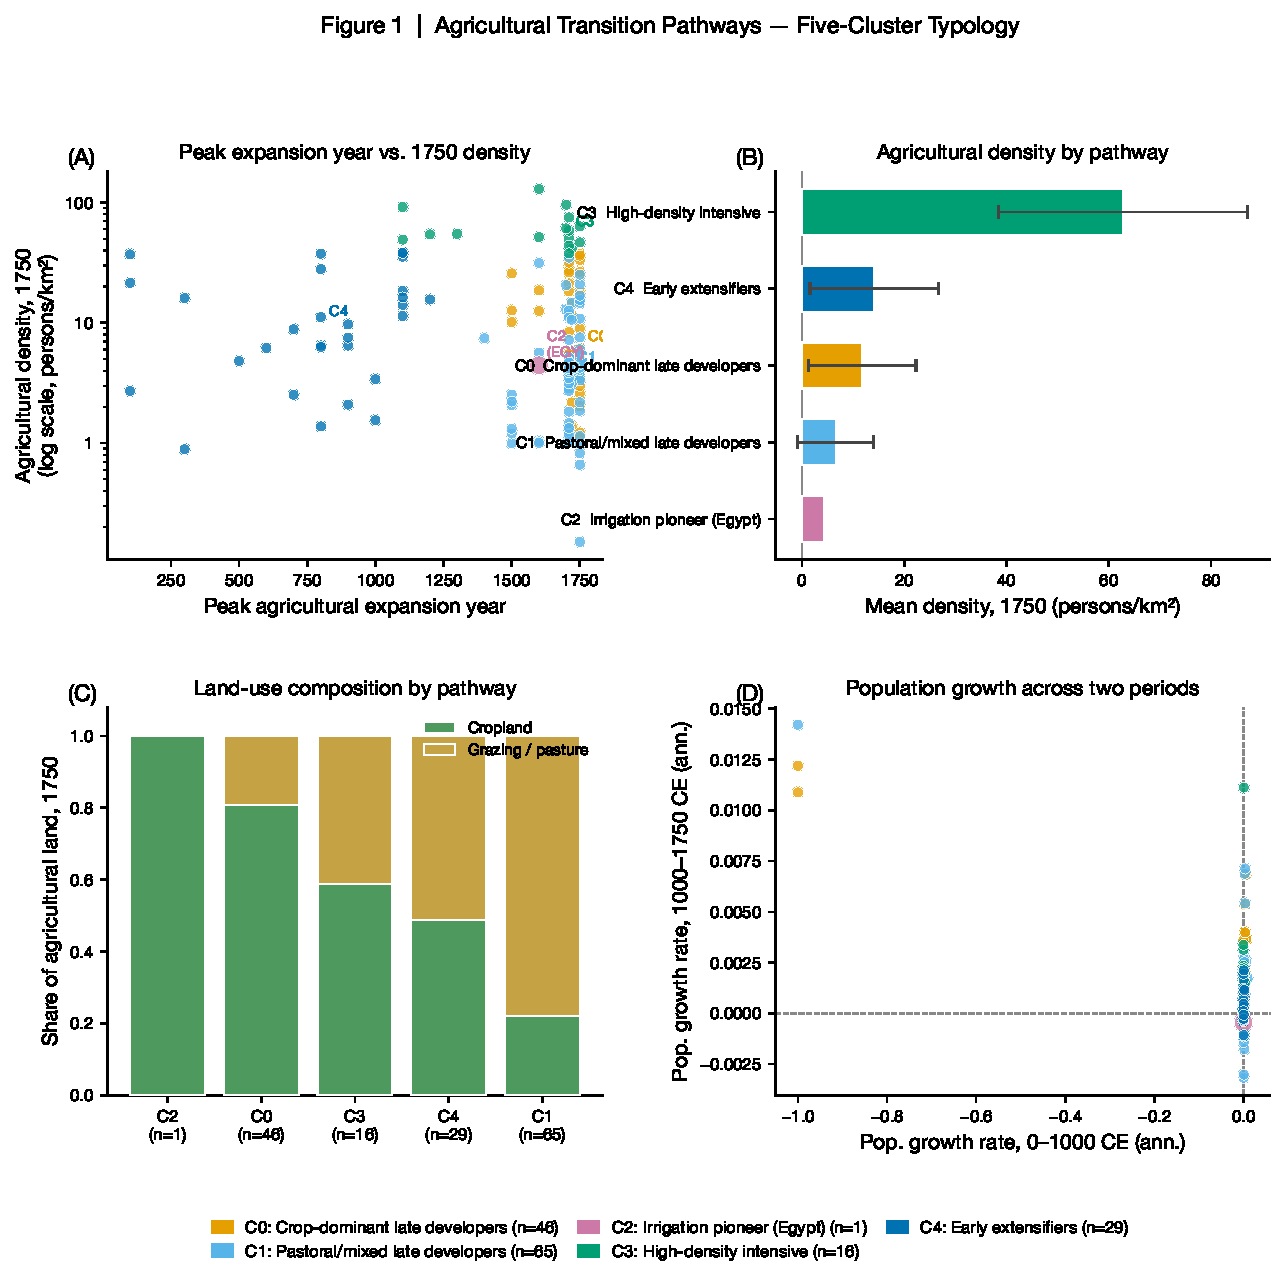
\includegraphics[width=\textwidth]{../analysis/figures/fig1_pathway_typology.pdf}
\caption{\textbf{Agricultural Transition Pathways.} (A)~Scatter of peak agricultural expansion year vs.\ 1750 density. (B)~Mean density by pathway. (C)~Land-use composition. (D)~Population growth across two periods. Five clusters identified via $K$-means on standardized trajectory features.}
\label{fig:typology}
\end{figure}

\begin{figure}[H]
\centering
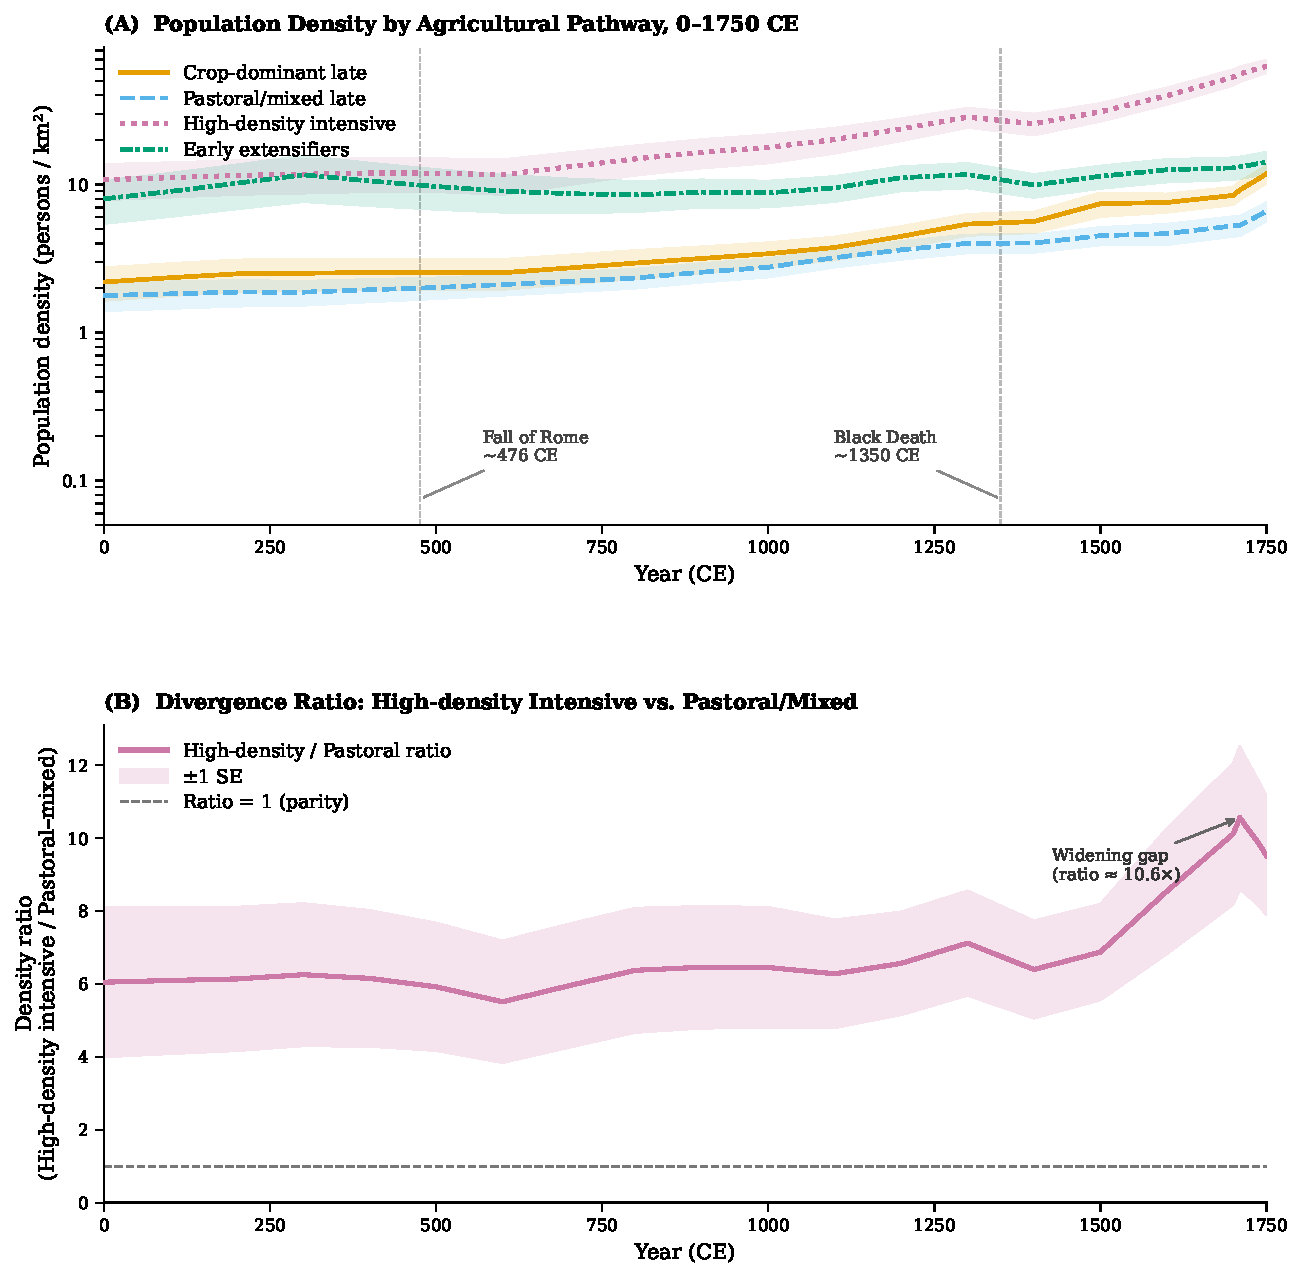
\includegraphics[width=\textwidth]{../analysis/figures/fig2_density_divergence.pdf}
\caption{\textbf{The Great Divergence in Population Density.} (A)~Population density trajectories by pathway, 0--1750~CE (log scale, $\pm$1~SE bands). (B)~Density ratio of high-density intensive to pastoral/mixed pathway, showing widening from $\sim$6$\times$ to $\sim$10$\times$.}
\label{fig:divergence}
\end{figure}

\begin{figure}[H]
\centering
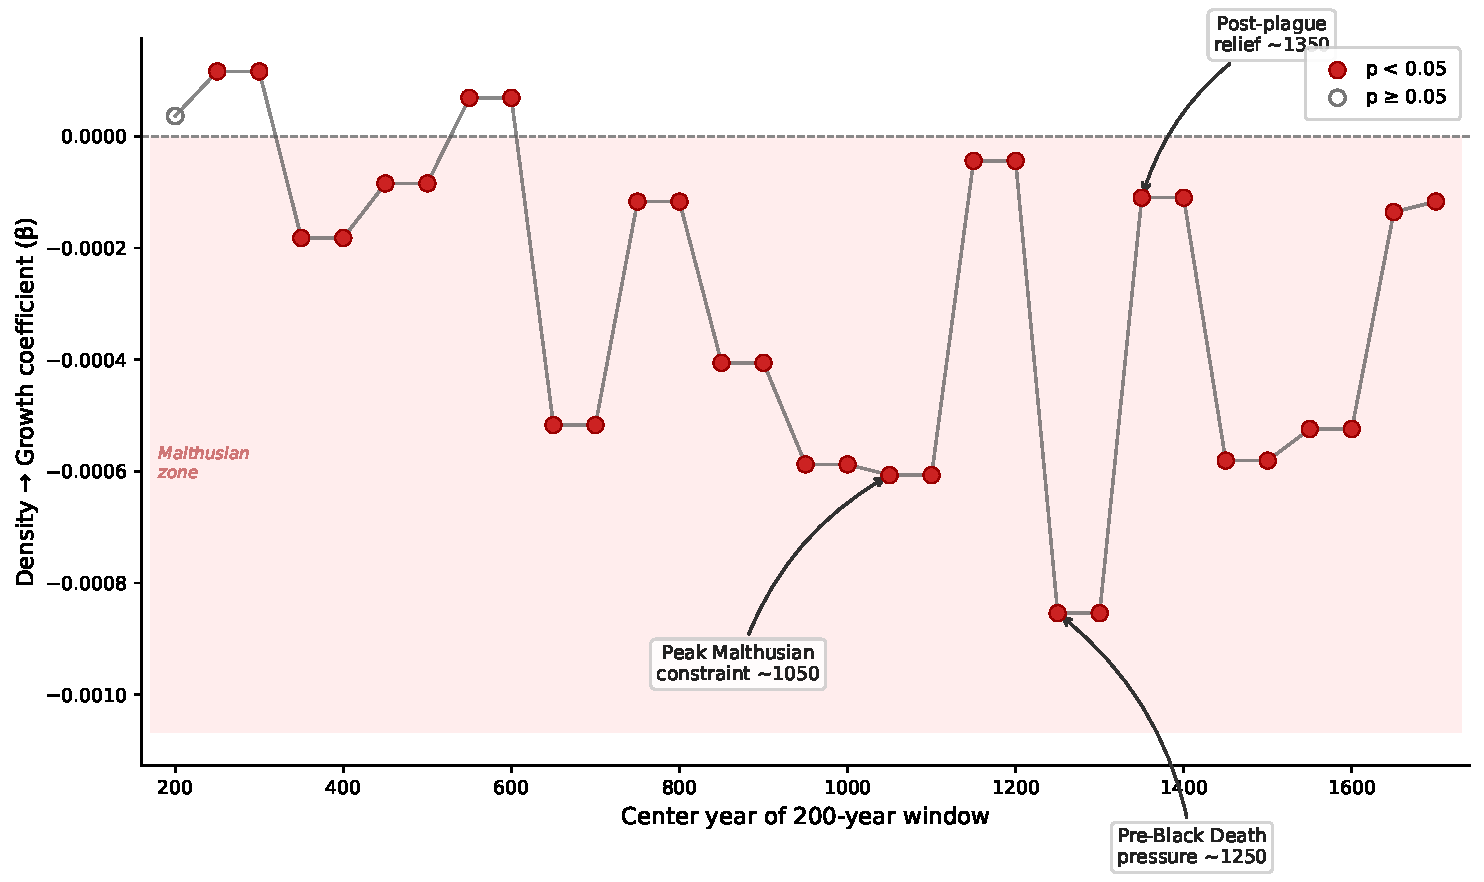
\includegraphics[width=\textwidth]{../analysis/figures/fig3_rolling_malthusian.pdf}
\caption{\textbf{Time-Varying Malthusian Coefficient.} Rolling 200-year window estimates of the density$\to$growth coefficient. Red dots indicate statistical significance ($p < 0.05$). Shaded region denotes the ``Malthusian zone'' ($\beta < 0$). Annotations mark peak constraint ($\sim$1050~CE), pre-Black Death pressure ($\sim$1250~CE), and post-plague relief ($\sim$1350~CE).}
\label{fig:rolling}
\end{figure}

\begin{figure}[H]
\centering
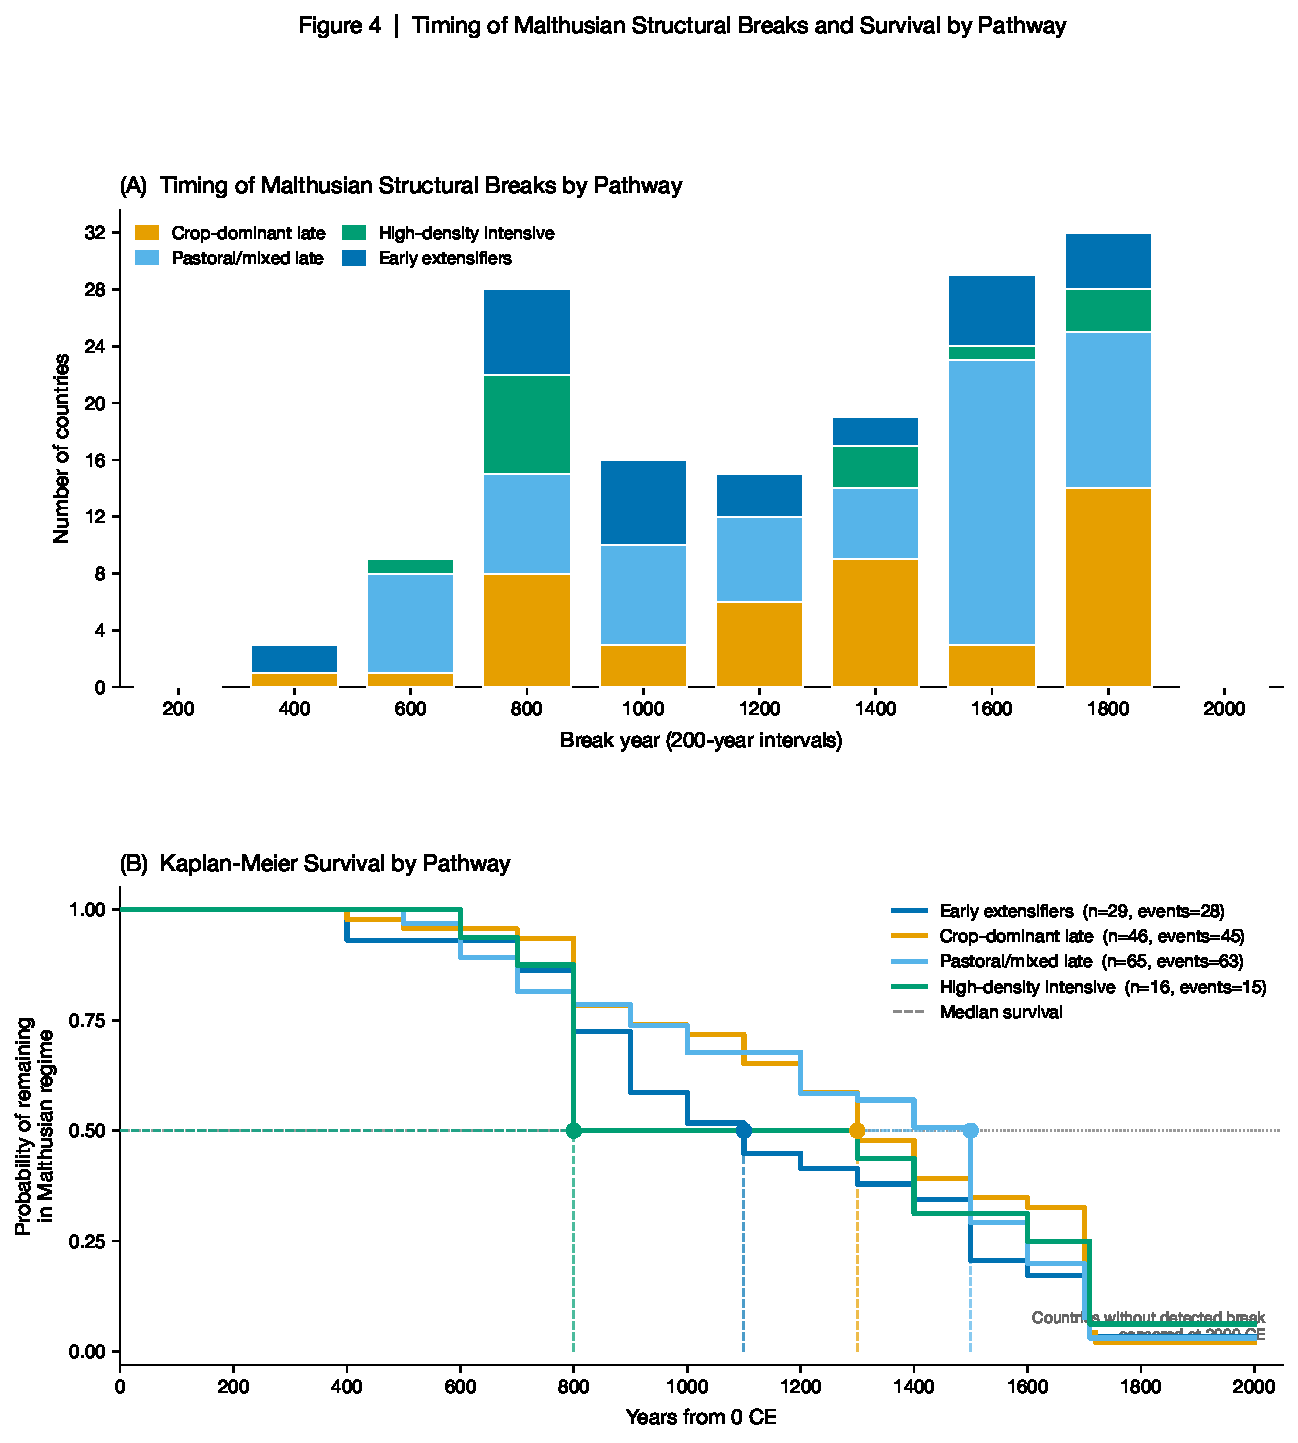
\includegraphics[width=\textwidth]{../analysis/figures/fig4_breaks_survival.pdf}
\caption{\textbf{Structural Breaks and Survival.} (A)~Histogram of earliest structural break year by pathway. (B)~Kaplan-Meier survival curves: probability of remaining in the Malthusian regime over time.}
\label{fig:breaks}
\end{figure}

\begin{figure}[H]
\centering
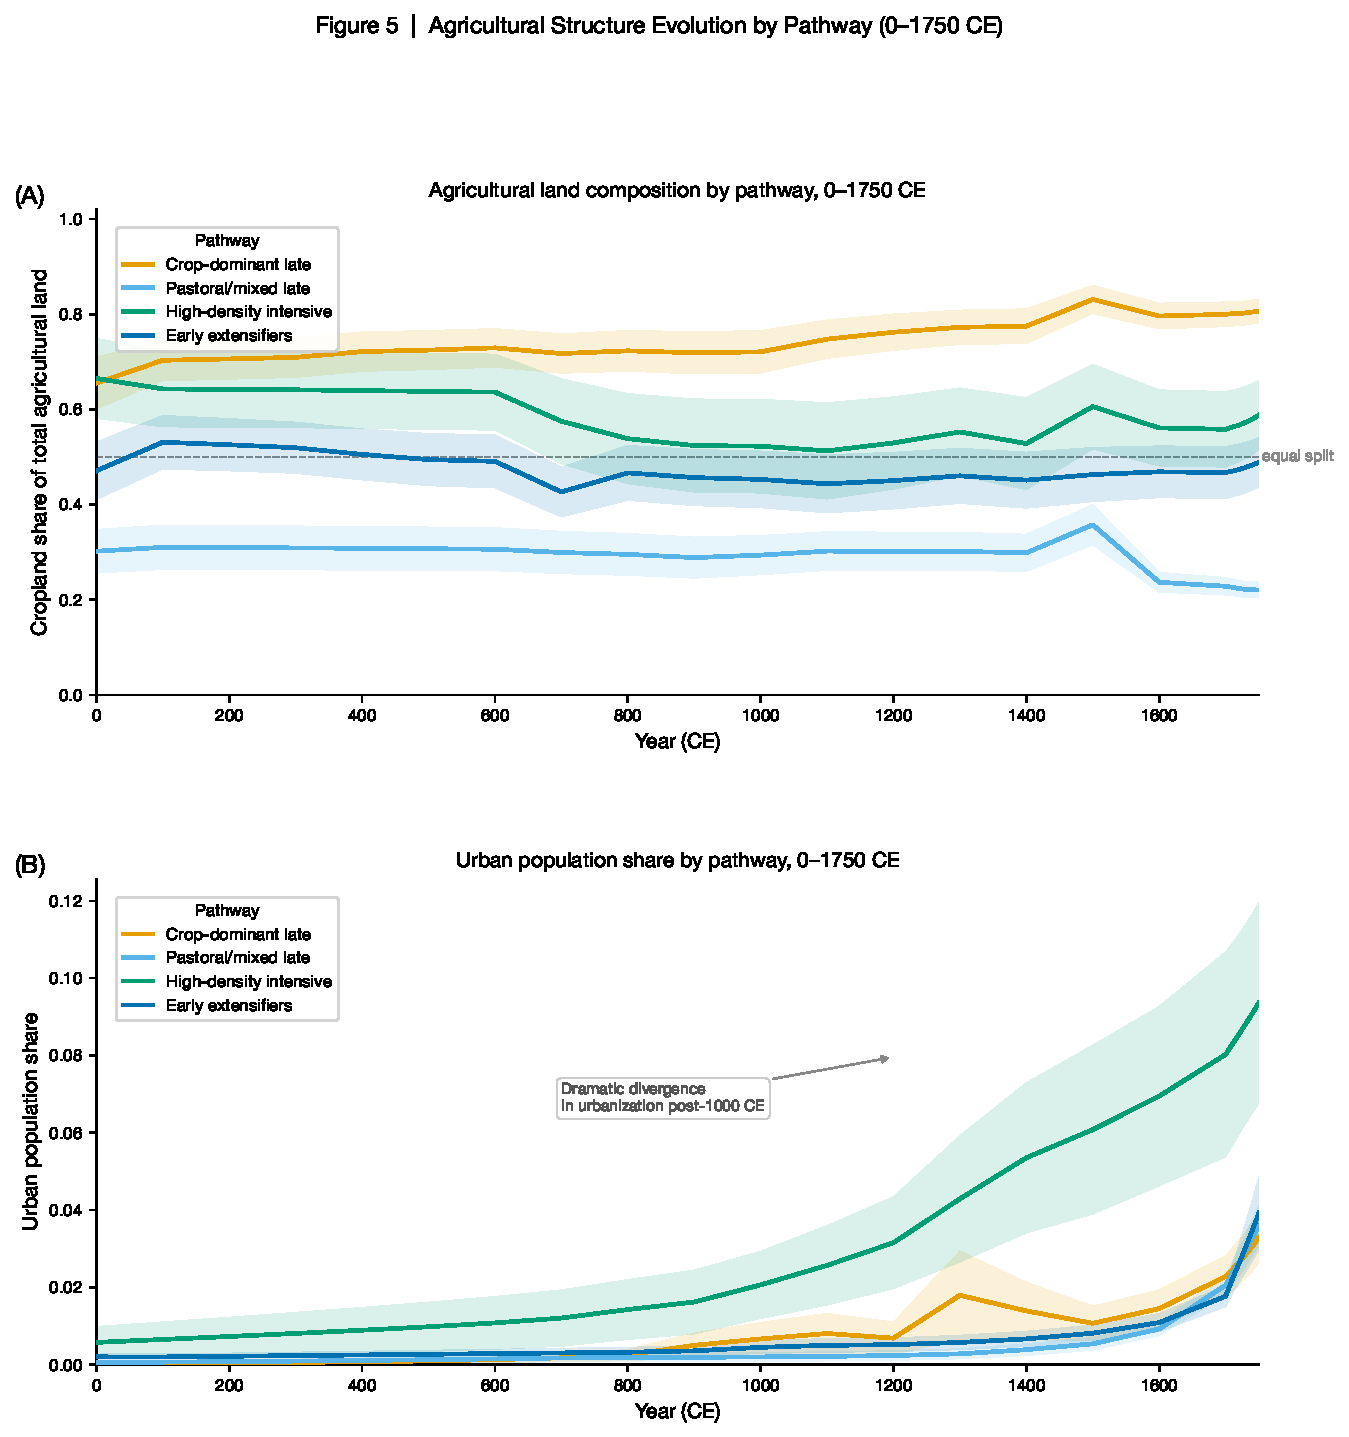
\includegraphics[width=\textwidth]{../analysis/figures/fig5_ag_structure_evolution.pdf}
\caption{\textbf{Agricultural Structure Evolution.} (A)~Cropland share of total agricultural land over time. (B)~Urban population share. Both show dramatic divergence across pathways after $\sim$1000~CE.}
\label{fig:ag_structure}
\end{figure}

\begin{figure}[H]
\centering
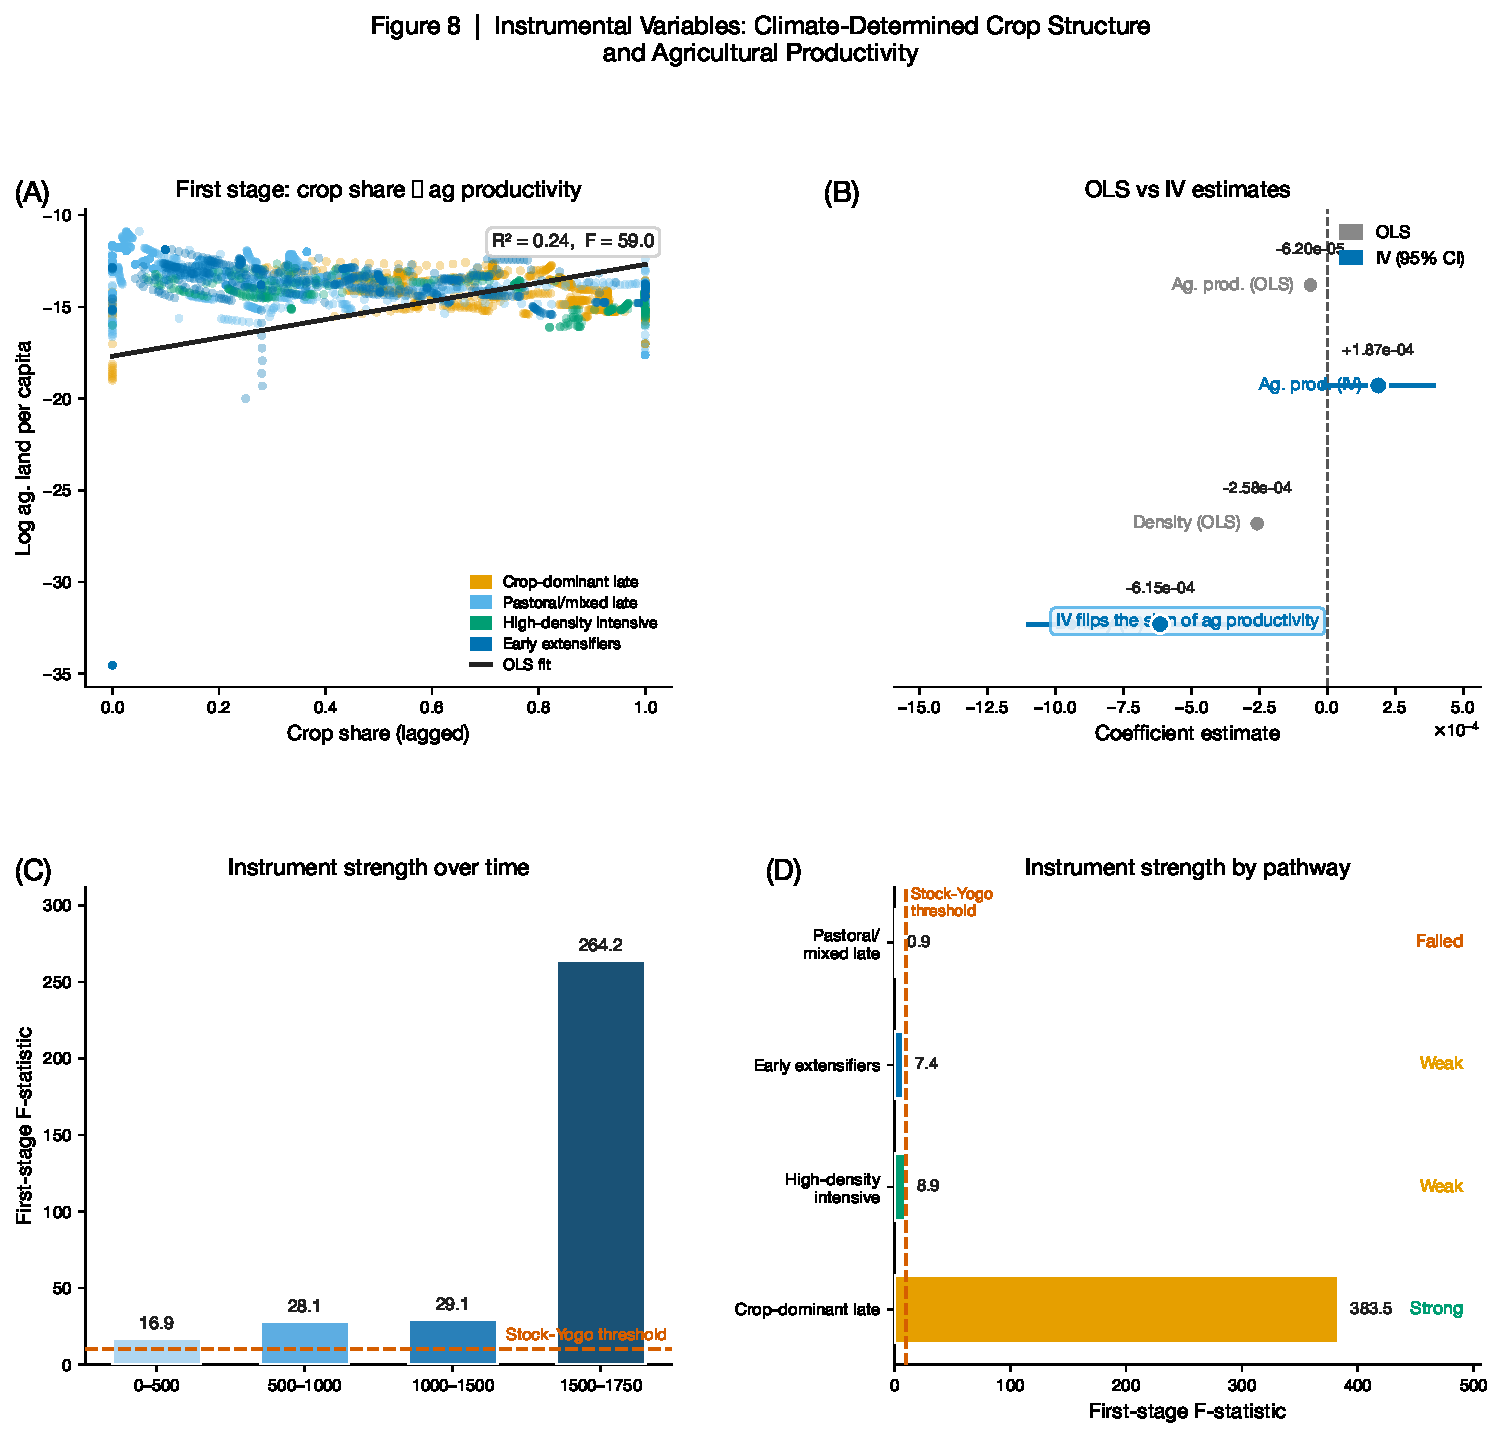
\includegraphics[width=\textwidth]{../analysis/figures/fig8_iv_identification.pdf}
\caption{\textbf{Instrumental Variables Identification.} (A)~First-stage scatter. (B)~OLS vs.\ IV coefficient comparison. (C)~Instrument strength by period. (D)~Instrument strength by pathway.}
\label{fig:iv}
\end{figure}

\begin{figure}[H]
\centering
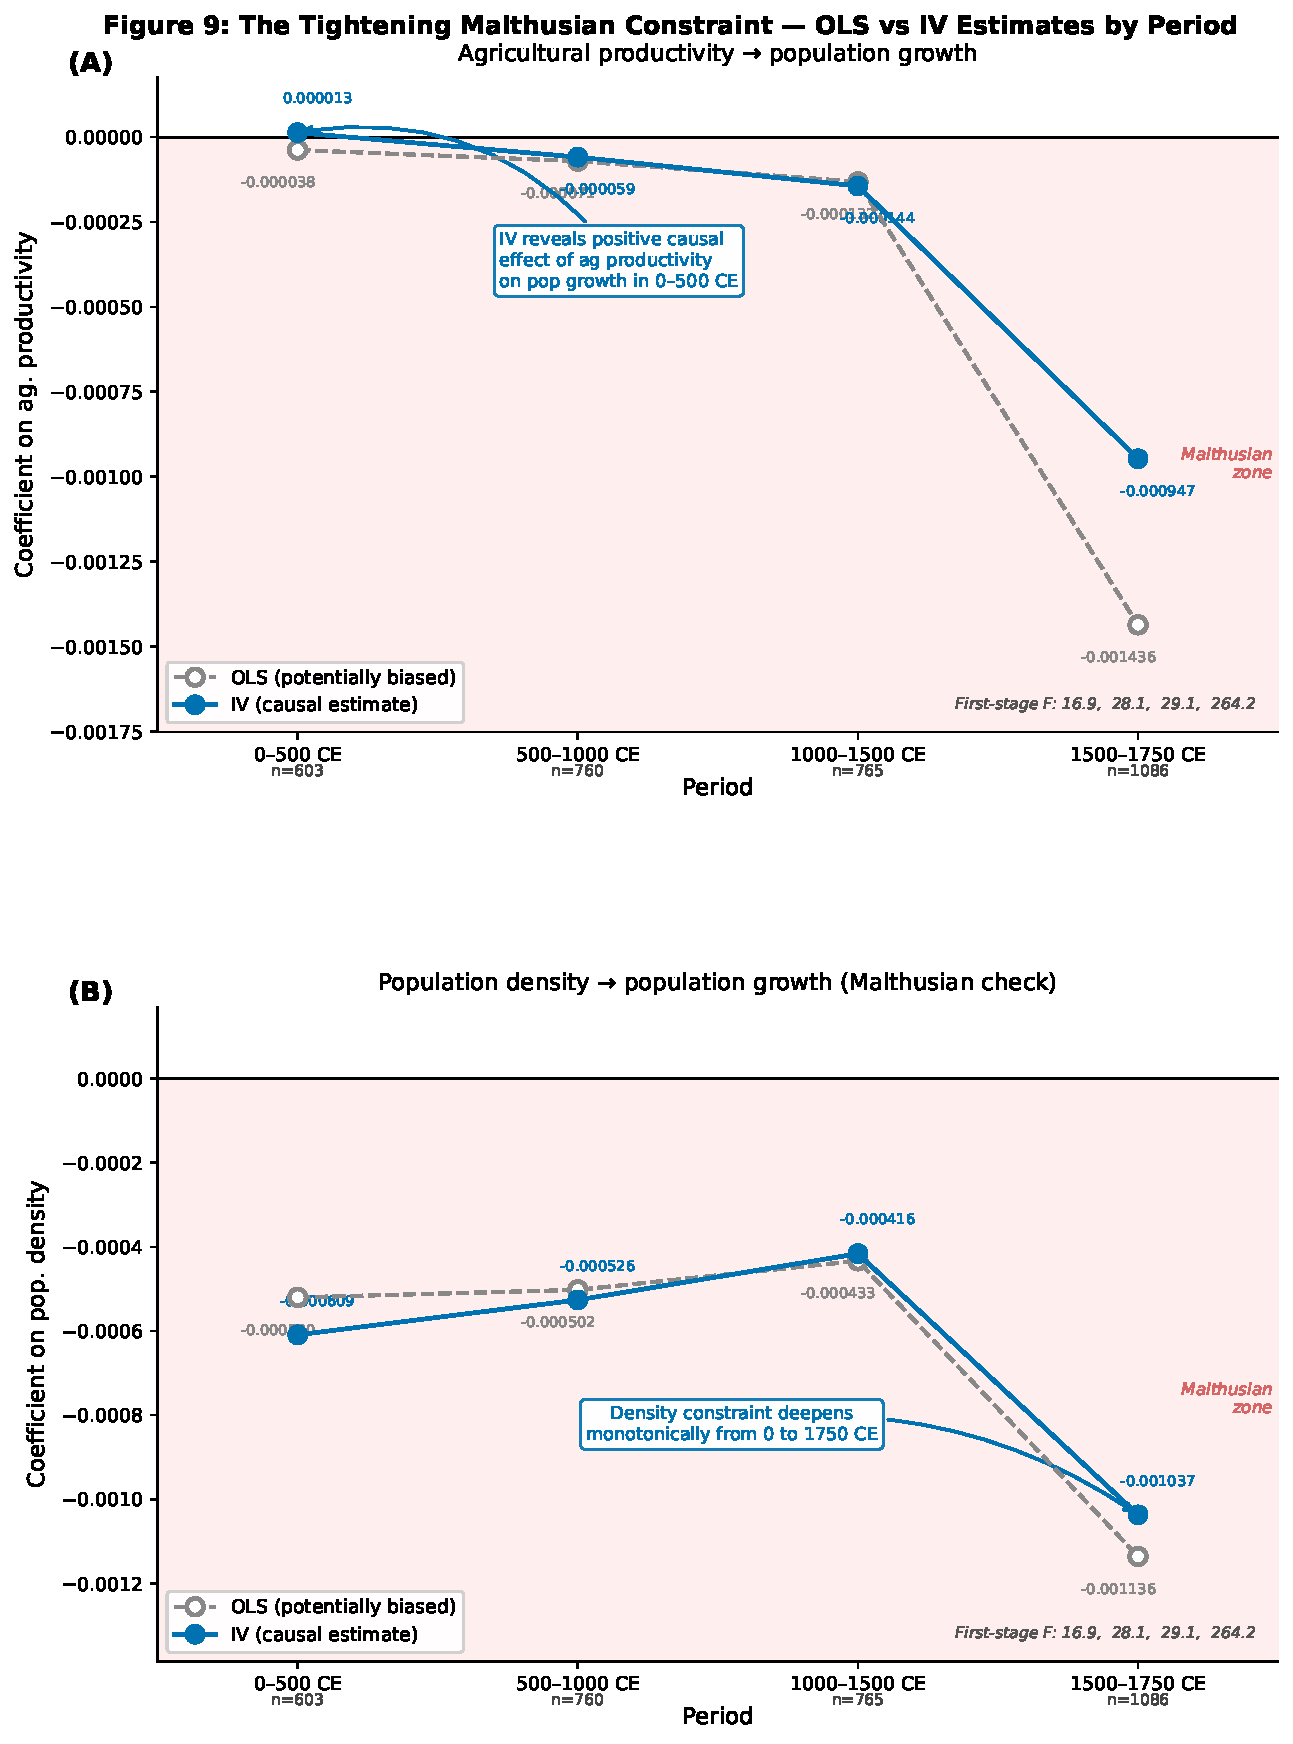
\includegraphics[width=\textwidth]{../analysis/figures/fig9_ols_vs_iv_periods.pdf}
\caption{\textbf{OLS vs.\ IV Estimates by Period.} (A)~Agricultural productivity effect: IV reveals positive causal effect in 0--500~CE masked by OLS bias. (B)~Density effect: consistently negative, deepening toward 1750.}
\label{fig:ols_iv}
\end{figure}

\begin{figure}[H]
\centering
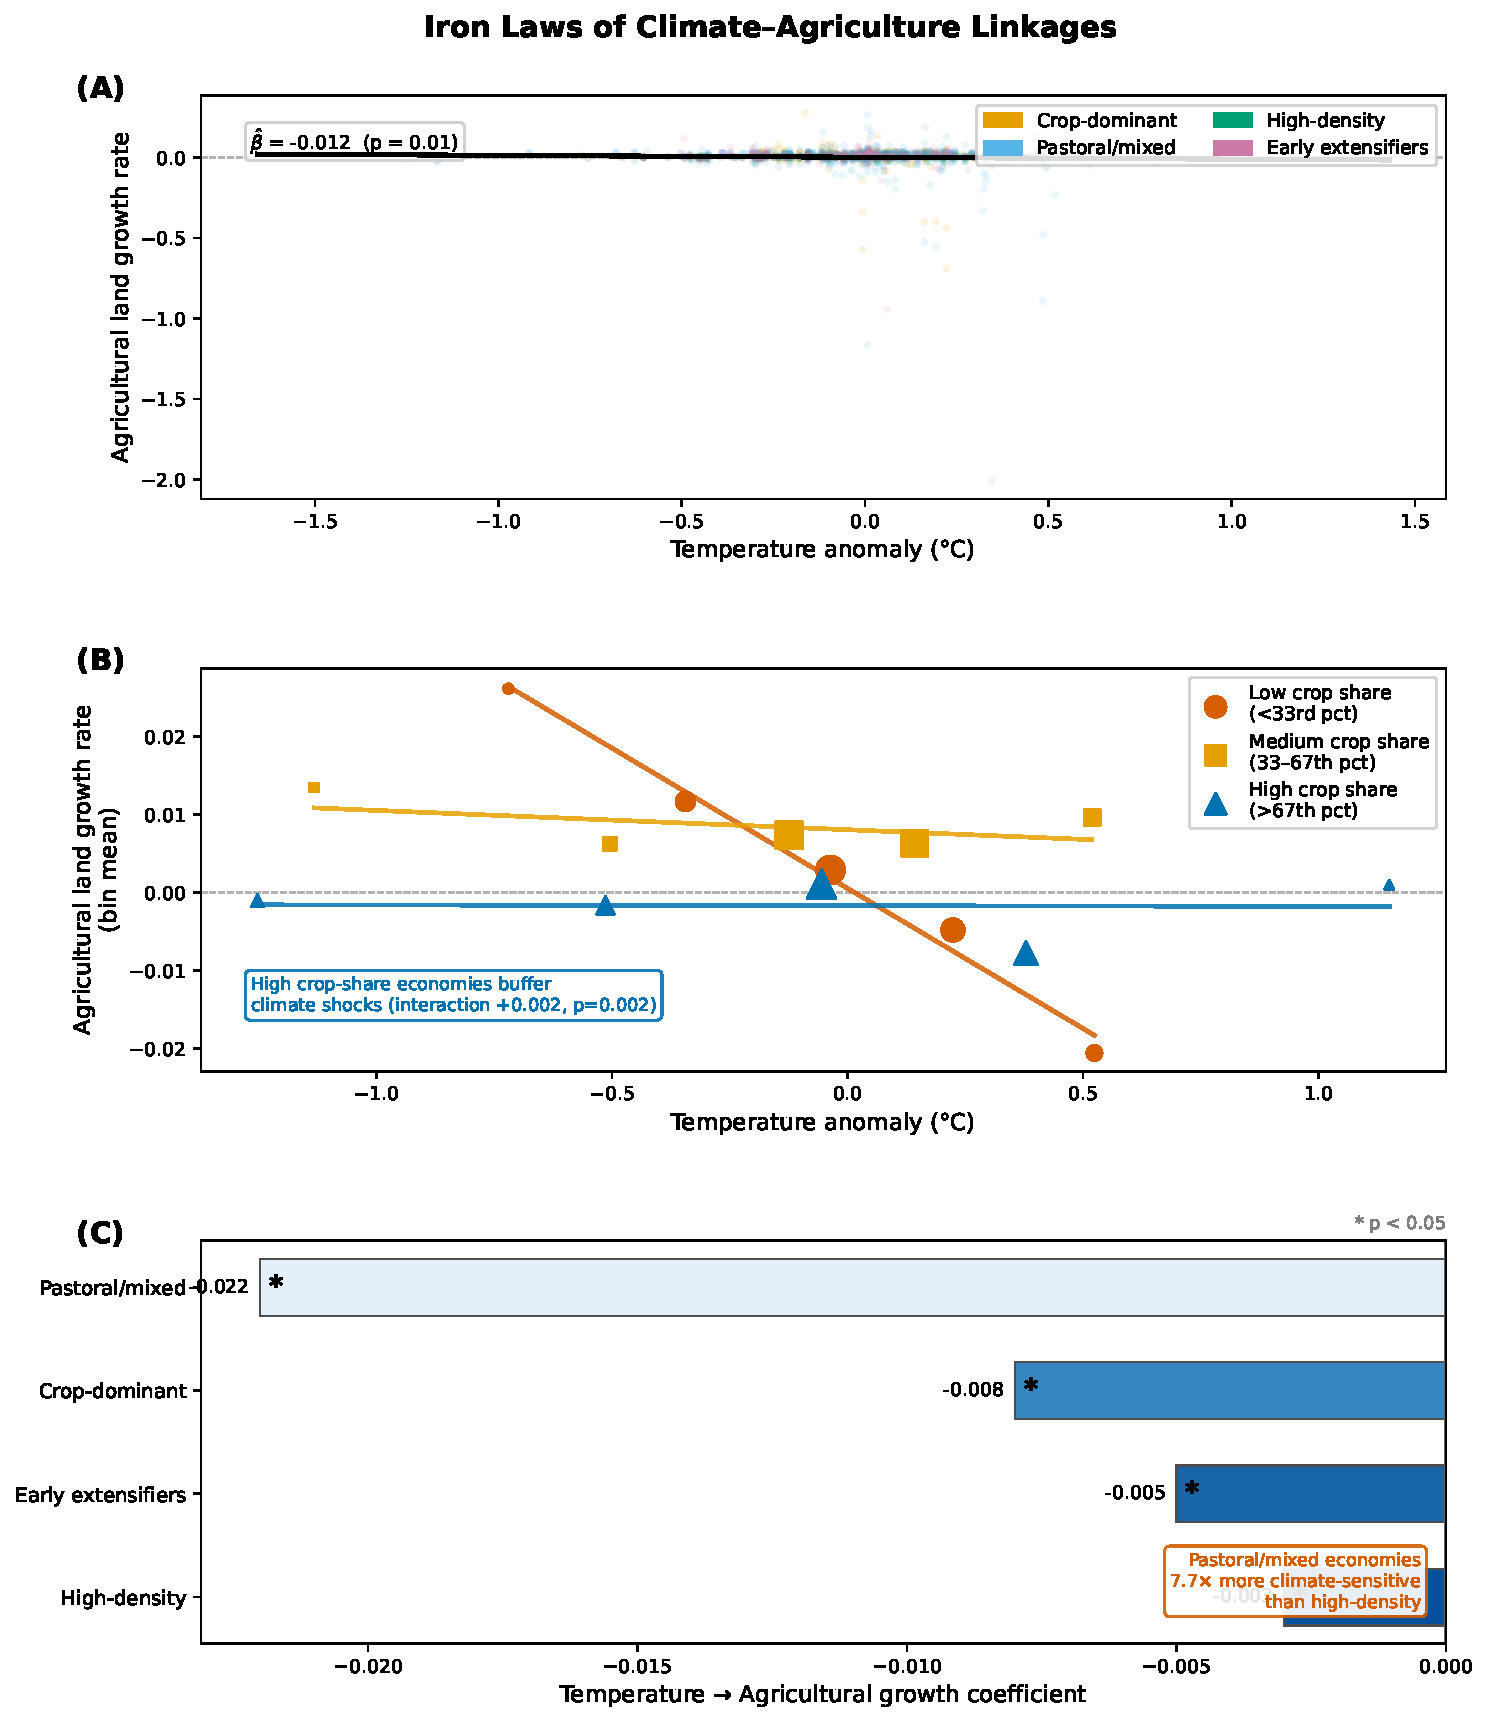
\includegraphics[width=\textwidth]{../analysis/figures/fig11_iron_laws.pdf}
\caption{\textbf{Iron Laws of Climate--Agriculture Linkages.} (A)~Temperature anomaly vs.\ agricultural growth. (B)~Buffering by crop share (binscatter by tercile). (C)~Climate sensitivity by pathway.}
\label{fig:iron_laws}
\end{figure}

\begin{figure}[H]
\centering
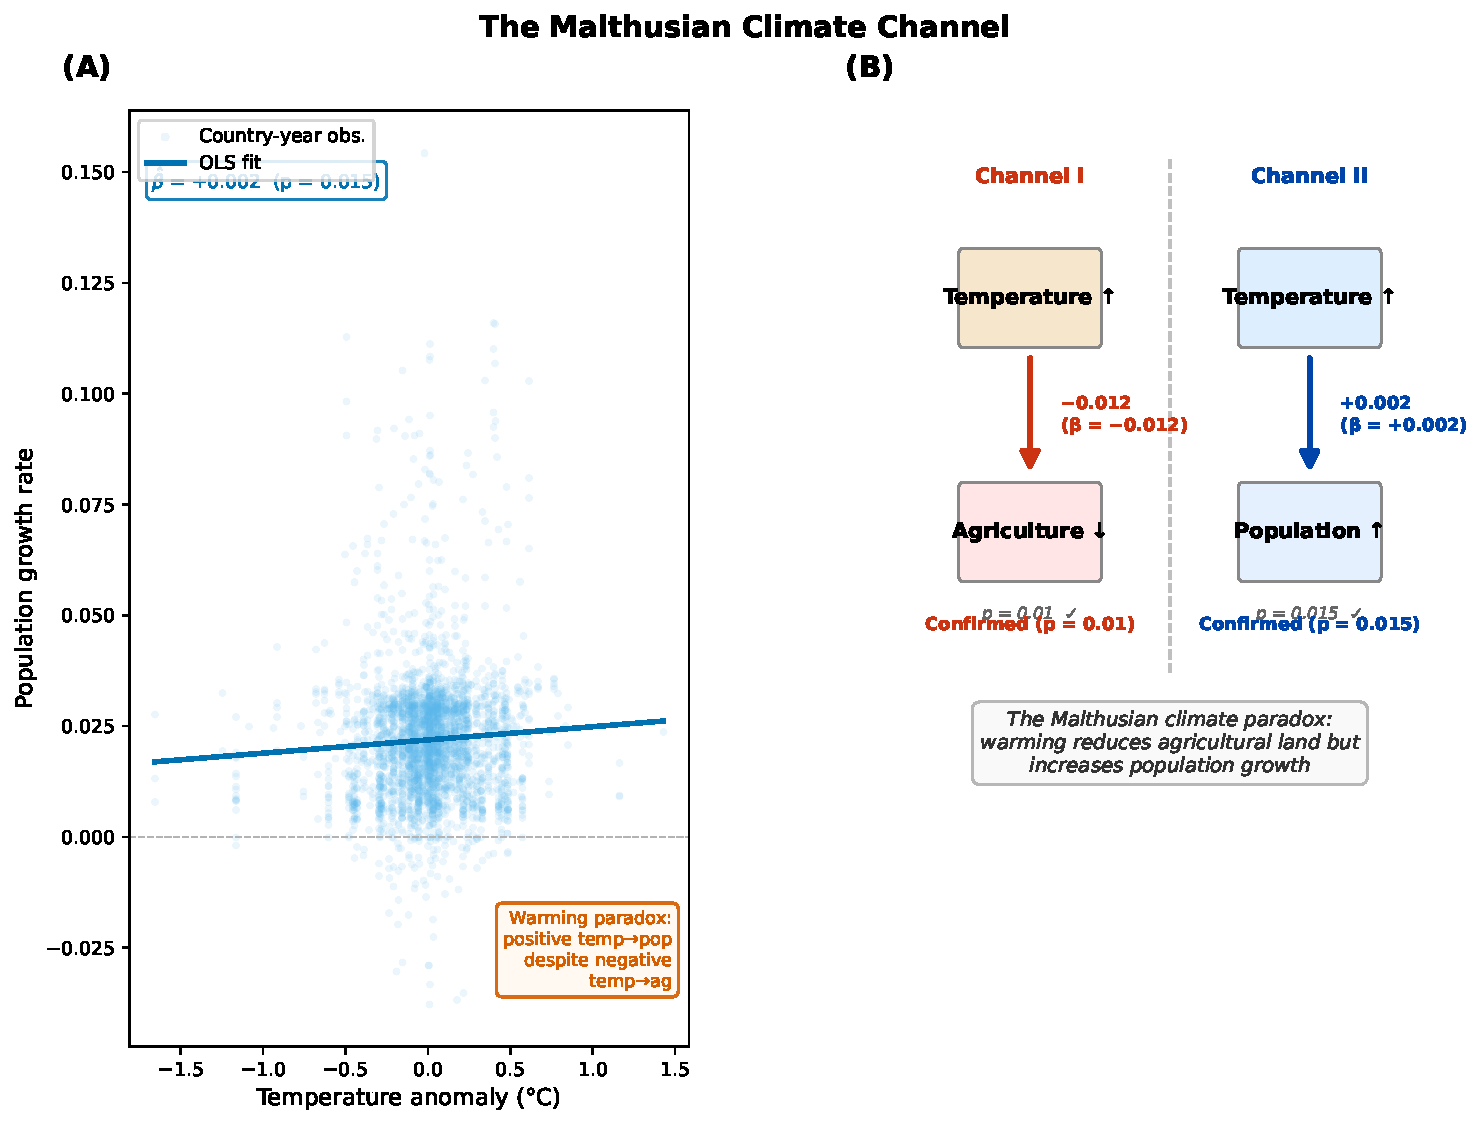
\includegraphics[width=\textwidth]{../analysis/figures/fig12_climate_channel.pdf}
\caption{\textbf{The Malthusian Climate Paradox.} (A)~Positive temperature--population relationship. (B)~Schematic of the dual channel: warming reduces agriculture but increases population.}
\label{fig:paradox}
\end{figure}

\end{document}
